\section{Ligas de alta entropia}\label{sec:LABEL_CHP_3_SEC_A}


Conhecidas também pelo termo inglês (HEAs - High-entropy alloys), são materiais altamente avançados que diferentemente das ligas convencionais, as HEAs possuem múltiplos elementos principais na liga, frequentemente cinco ou mais elementos de peso e raio atômico quase iguais. O princípio básico por trás de uma HEA é a capacidade das fases de solução sólida serem relativamente estáveis, devido a sua alta entropia de mistura, a estabilização da solução sólida é significativamente maior do que a formação de intermetálicos. Basicamente as HEAs contém ao menos cinco elementos e a composição atômica de cada elemento varia entre 5\% e 35\%. \cite{yeh2013alloy} \cite{yeh2004nanostructured}

\begin{figure}[ht]
    \centering
    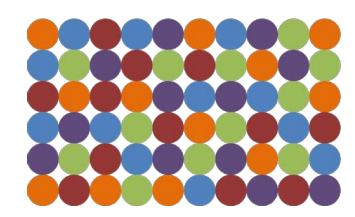
\includegraphics{esquema-ligas-hea.png} 
    \caption{Esquema de uma liga de alta entropia composta por cinco elementos em matriz de solução sólida}
    \label{fig:esquema-ligas-hea}
\end{figure}


Baseando-se na equação de Boltzmann \cite{gaskell2012introduction}, relacionando a entropia e a complexidade do sistema \cite{thermodynamicsOfSolid}, a mudança de entropia configuracional por mol, $\Delta S_{config}$, durante a formação de uma solução  de n elementos com frações equimolares pode ser calculada a partir da seguinte equação:

\begin{equation}
    \Delta S_{config} = k \ln \omega
\end{equation}

onde k é a constante de Boltzmann e $\omega$ é a medida de aleatoriedade para energia disponível na mistura ou dispersa entre as partículas de um sistema. Assim a entropia configuracional em função do número de moles de uma solução sólida de n elementos com fração molar de $x_i$ é:

\begin{equation}
    \Delta S_{config} = - R \sum_{i=1}^{n} X_{i} \ln X_{i}
\end{equation}

Considerando uma liga equiatômica no estado líquido ou em uma solução sólida regular. A entropia configuracional por mol é dada pela Equação \ref{eq:boltzmman-complexidade} \cite{yeh2004nanostructured} \cite{yeh2013alloy}:
\begin{equation} 
\Delta S_{config} = - k \ln \omega = - R (\frac{1}{n} \ln \frac{1}{n} + \frac{1}{n} \ln \frac{1}{n} + ... + \frac{1}{n} \ln \frac{1}{n}) = -R \ln \frac{1}{n} = R \ln n
\label{eq:boltzmman-complexidade}
\end{equation}

Onde R é a contante dos gases igual a $8,314J/K^{-1}mol^{-1}$.  Pela regra de Richard \cite{thermodynamicsOfSolid}, as mudanças de entropia na fusão da maioria dos metais são apenas empiricamente igual a R em seus pontos de fusão.
A entropia configuracional de ligas equiatômicas em função dos elementos principais é demonstrado na tabela \ref{quad:entropia-config-n} e na figura \ref{fig:entropia-configuracional-elementos}.


\begin{table}[htb]
\centering
\caption{Entropia configuracional de ligas equimolares para n elementos}
\begin{supertabular}{|m{1.5cm}|m{1.5cm}|m{1.5cm}|m{1.5cm}|m{1.5cm}|m{1.5cm}|m{1.5cm}|m{1.5cm}|}
\hline
{ n } &
{ 1 } &
{ 3 } &
{ 5 } &
{ 7 } &
{ 9 } &
{ 11 } &
{ 13 }\\\hline
{ $\Delta S_{config}$ } & 
{ 0 } &
{ 1,10R } &
{ 1,61R } &
{ 1,95R } &
{ 2,20R } &
{ 2,40R } &
{ 2,57R} \\\hline
\end{supertabular}
    \legend{}
    \label{quad:entropia-config-n}
\end{table}

\begin{figure}[ht]
    \centering
    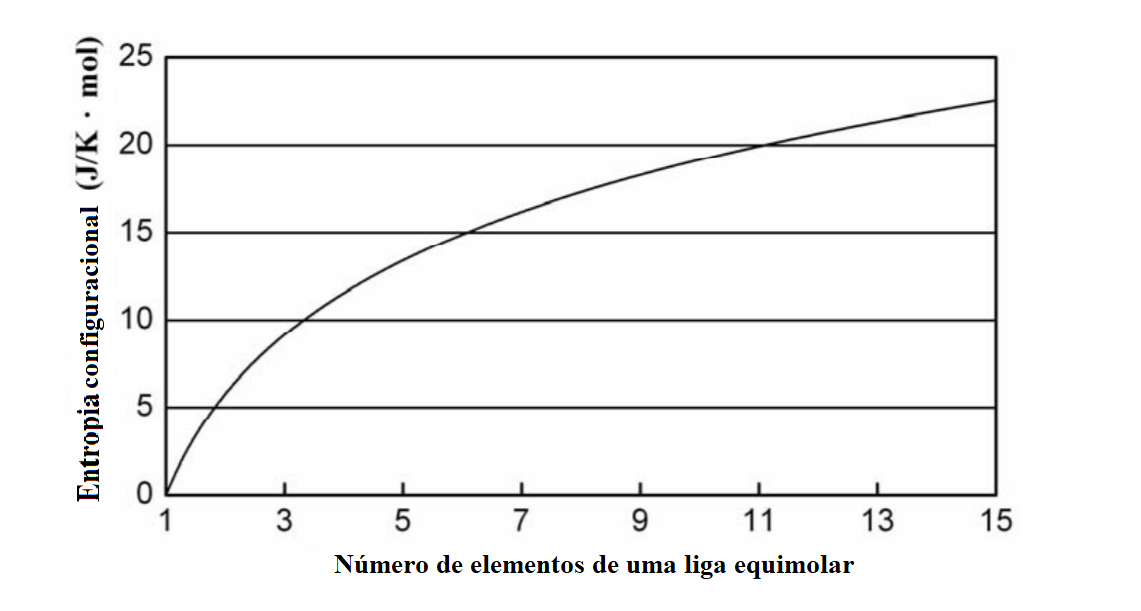
\includegraphics[height=6cm]{entropia-mistura-numero-elementos.png} 
    \caption{Entropia configuracional em função do número de elementos para ligas equimolares. Adaptado de \cite{jien2006recent}.}
    \label{fig:entropia-configuracional-elementos}
\end{figure}

Por convenção, uma liga é considerada de alta entropia quando possui a entropia configuracional maior que 1,5R. sendo assim uma liga de alta entropia é classificada conforme a figura \ref{fig:divisao-ligas-alta-entropia} \cite{gao2016high}:

\begin{figure}[ht]
    \centering
    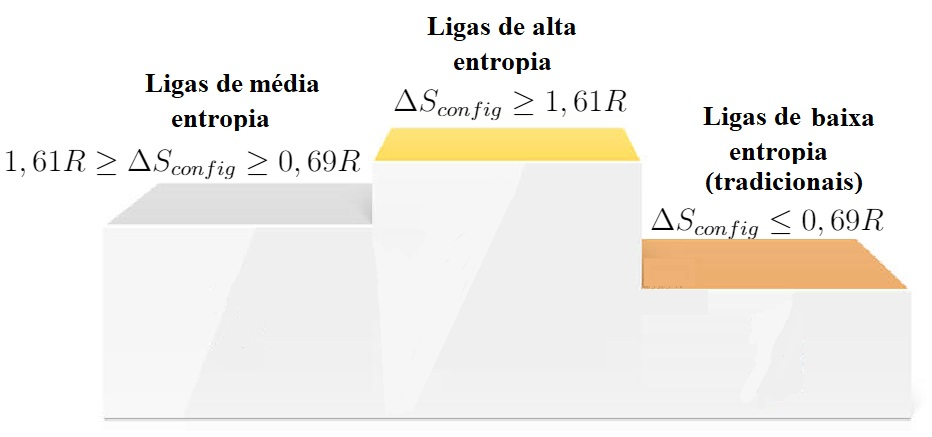
\includegraphics[height=6cm]{divisao-ligas-alta-entropia.jpg} 
    \caption{Divisão das ligas baseado na entropia configuracional.}
    \label{fig:divisao-ligas-alta-entropia}
\end{figure}
     
\pagebreak
                   
\subsection{Efeitos principais em Ligas de Alta Entropia}\label{sec:LABEL_CHP_3_SEC_B_SUB_A}

Em ligas de alta entropia, existem muitos fatores que afetam a microestrutura e as suas propriedades. Dentre estes diversos fatores, quatro deles se destacam \cite{yeh2013alloy}, são eles a alta entropia, distorção severa da rede, difusão retardada e efeito coquetel \cite{gao2016high} \cite{murty2019high}.

\subsection{Alta Entropia}\label{sec:LABEL_CHP_3_SEC_B_SUB_B}

É o efeito mais importante em Ligas de Alta Entropia, este contribui com o aumento da formação de fases em solução sólida, tornando a microestrutura muito mais simples do que a conhecida em ligas convencionais. Há três categorias de estados concorrentes no estado sólido de uma liga, isto é, fases elementares, compostos intermetálicos e fases de solução sólida. 
A competição envolvendo a fase líquida durante a solidificação não é considerada. A fase elemental é a fase terminal de uma solução sólida baseada em um único elemento metálico. 
Compostos intermetálicos são compostos estequiométricos que possuem super redes específicas, como NiAl e Ni$_{3}$ Ti. Solução sólida é a fase de mistura completa de todos os elementos ou com uma mistura significante em que elementos constituintes da liga apresentam a mesma estrutura cristalina. Fases intermetálicas ou intermediárias estão inclusas também porque são solidas baseadas em componentes intermetálicos. Nessas fases, diferentes elementos constituintes tendem a ocupar diferentes conjuntos de locais de rede. De acordo com a Segunda lei da Termodinâmica, o estado com a menor energia livre de mistura $\Delta G_{mix}$ entre todos os possíveis estados deve estar em estado de equilíbrio. 
Em resumo, o efeito de alta entropia é importante para Ligas de Alta Entropia para evitar a formação de muitos tipos diferentes de compostos estequiométricos, que são muito frágeis e complexos. Por outro lado, promove a formação de solução sólida, reduzindo o número de fases conforme previsto pela regra de fase de Gibbs, que permite que o número de fases em equilíbrio aumente com o número de componentes. \cite{yeh2013alloy}


% A figura 1 abaixo representa o diagrama ternário da entropia de mistura de um sistema de uma liga ternária $\Delta S_{mix}(J.mol^{-1}K^{-1})$. As regiões de cor azul indicam a presença de ligas convencionais baseadas em um ou dois elementos principais, e a região vermelha do centro indica  alta entropia.

% \begin{figure}[ht]
%     \centering
%     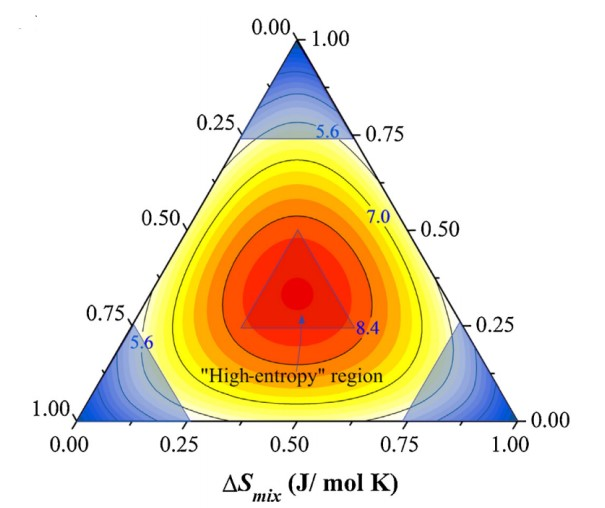
\includegraphics[width=8.5cm,height=7.5cm]{diagrama-ternario-de-entropia.jpg}
%     \caption{Esquema de um sistema de liga ternária . Adaptado de  \cite{ye2016high}}
%     \label{fig:internet}
% \end{figure}




\subsection{Distorção severa na rede}\label{sec:LABEL_CHP_3_SEC_B_SUB_C}

Devido a uma matriz multielementar, cada fase em solução sólida em uma Liga de Alta Entropia é uma  inteiramente composta por solutos \cite{tong2005mechanical}, onde cada átomo está rodeado por diferentes tipos de elementos, e consequentemente, apresentando tensões e deformações na rede devido a diferença de raio atômico entre  eles.

Além da diferença de raio atômico, tanto a diferença de energia de ligação quanto a tendencia de estrutura cristalina entre os elementos constituintes também podem causar distorções ainda maiores na rede, isto porque as ligações não simétricas e a estrutura eletrônica estão presentes entre um átomo e seus primeiros vizinhos, além dessa assimetria variar de local para local na rede.\cite{tsai2013sluggish}\cite{yeh2007anomalous} 

\begin{figure}[ht]
    \centering
    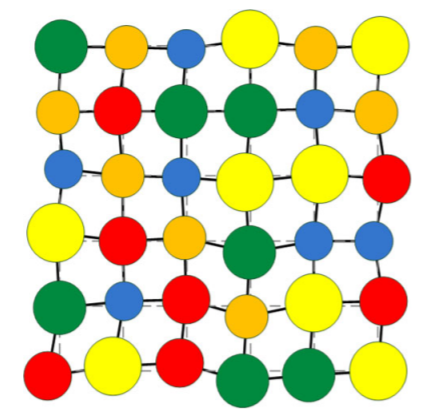
\includegraphics[width=8.5cm,height=7.5cm]{distorcao-severa-rede.png} 
    \caption{Distorção severa na rede cristalina devido a diferença de tamanho e energia de ligação dos elementos. Adaptado de \cite{yeh2013alloy}}
    \label{fig:internet}
\end{figure}

A gravidade do efeito da distorção na rede é significativamente maior em ligas de alta entropia, quando comparadas as ligas convencionais, isto porque em ligas convencionais a maioria dos átomos da matriz possuem o mesmo tipo de átomos em sua vizinhança.

Segundo \cite{yeh2013alloy} essa distorção não afeta apenas as propriedades, como também reduz o efeito térmico sobre a liga. A dureza e a resistência mecânica aumentam efetivamente devido ao grande endurecimento da solução na rede fortemente distorcida. Foi observado que ligas com a estrutura CFC são menos endurecíveis por solução sólida quando comparadas a ligas com estrutura CCC \cite{brooks1982heat}. Na estrutura CFC, cada átomo é cercado por 12 átomos vizinhos, por outro lado, na estrutura CCC, cada átomo é cercado por 8 átomos. Dessa maneira, considerando a o mesmo conjunto de elementos, um átomo na estrutura CFC terá maior probabilidade de estar ligado com o mesmo elemento, resultando, assim, em menor endurecimento e menor distorção na rede\cite{dieter1976mechanical}.

Outro fenômeno que vale ressaltar é a queda significativa da condutividade elétrica observada em ligas de Alta Entropia, isto ocorre por causa do espalhamento de elétrons ocasionado pela distorção da rede. Que por consequência influi na redução da condutividade térmica \cite{kao2011electrical}.

% \begin{figure}[ht]
%     \centering
%     \caption{Distorção severa em rede de uma estrutura cristalina multielementar}
%     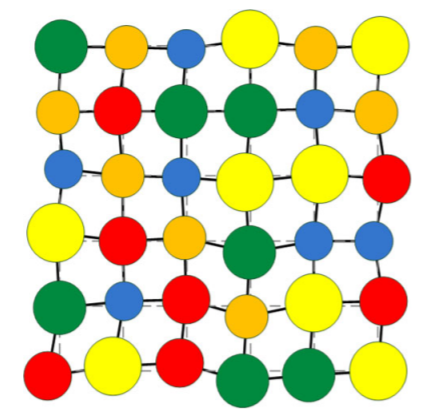
\includegraphics{distorcao-severa-rede.png} 
%     \legend{Fonte: Yeh, Alloy design strategies and future trends in high-entropy alloys (2013, p. 1764)}
%     \label{fig:internet}
% \end{figure}


\pagebreak

\subsection{Difusão lenta}\label{sec:LABEL_CHP_3_SEC_B_SUB_D}

Em ligas de alta entropia, a concentração de lacunas na rede é limitada quando comparado a ligas tradicionais, isso porque cada lacuna está associada a entalpia positiva de formação e excesso de entropia de mistura, na qual gera uma mínimo de energia livre de mistura a uma certa concentração de equilíbrio para uma dada temperatura. \cite{thermodynamicsOfSolid}


Uma lacuna em uma solução sólida é rodeada e competida por átomos de diferentes elementos durante a difusão. Foi proposto que a difusão mais lenta e alta energia de ativação ocorre em Ligas de Alta Entropia devido à grande flutuação da energia potencial da rede entre os locais da rede. É considerado que a difusão lenta e a alta energia de ativação pode ocorrer em HEAs devido a abrangente variação da energia potencial da rede entre sítios da rede.\cite{tsai2013sluggish}. Tudo isso, somado à distorção severa da rede, a qual limita a movimentação atômica, resultando numa taxa de difusão limitada em ligas de alta entropia \cite{jien2006recent}.

Devido ao efeito de difusão lenta, vantagens são fornecidas pelo fato de afetar diretamente na nucleação, crescimento de grão de forma mais lenta, precipitados nanométricos, temperatura de recristalização elevada e aumento da resistência a fluência. Essas vantagens trazem benefícios para o controle da microestrutura \cite{gao2016high}.


\subsection{Efeito coquetel}\label{sec:LABEL_CHP_3_SEC_B_SUB_E}

O termo ``coquetel multimetálico'' foi utilizado na literatura para enfatizar o aprimoramento das propriedades das ligas metálicas através da utilização de cinco ou mais elementos principais. Esse efeito indica que propriedades inesperadas podem ser
obtidas através da combinação de múltiplos elementos em uma liga, propriedades essas
que não poderiam ser obtidas em ligas baseadas em um único elemento principal

Apesar de sua grande tendência em possuir microestrutura monofásica, ligas de alta
entropia podem apresentar mais de uma fase, dependendo de sua composição e rota de 
processamento. Como em qualquer liga metálica, suas principais propriedades são
ditadas pelas fases que a constituem, através do efeito da morfologia, distribuição,
contornos e propriedades dessas fases. Cada fase consiste em uma solução sólida
multielementar, que pode ser definida como um compósito se analisada em escala
nanométrica. As propriedades desse compósito são regidas não somente pelas
propriedades básicas de cada elemento, mas também pela interação entre os mesmos e
pela distorção severa da rede. De maneira geral, o efeito coquetel vai desde a escala
atômica, através do efeito de compósito multielementar, até a escala micrométrica, pelo
efeito de multifases.

